\documentclass{beamer}

\usepackage{polski}
\usepackage[T1]{fontenc}
\usepackage[utf8]{inputenc}

\usepackage[polish]{babel}

\usepackage{subfig}
\usepackage{rotating}

\usetheme[backgroundimagefile=kosmos.jpg,opacity=0.6]{diepen}

\title{Symulacja układu planetarnego na GPU przy użyciu CUDA i OpenGL}
\subtitle{część pierwsza}
\author{Daniel Kłobuszewski\and Jakub Kotur}
\institute{Politechnika Warszawska}
\date{\today}

\begin{document}

\frame[plain]{\titlepage}

\frame{
	\frametitle{Treść prezentacji}
	\tableofcontents
}

\section{Opis technologii}\label{sec:opis technologii}


\subsection{CUDA}\label{sub:cuda}
\frame{ \frametitle{CUDA} \tableofcontents[currentsubsection] }

\frame
{
	\frametitle{CUDA}
}

\subsection{OpenGL}\label{sub:opengl}
\frame{ \frametitle{OpenGL 3.2} \tableofcontents[currentsubsection] }

\frame
{
	\frametitle{Jednostki cieniowania}

	Programowalne jednostki cieniowania (shadery):

	\begin{description}
	\item[vertex] - wykonywane dla każdego wierzchołka
	\item[fragmet] - wykonywane dla każdego piksela
	\pause
	\item[geometry] - wykonywane dla każdej figury (np. trójkąt, linia)
	\end{description}

}

\frame
{
	\frametitle{Vertex Shader}
	\begin{block}{Wejście}
	\begin{itemize}
	\item pozycja (przestrzeń modelu)
	\item kolor wierzchołka
	\item koordynaty tekstury
	\end{itemize}
	\end{block}
	\begin{block}{Wyjście}
	\begin{itemize}
	\item pozycja (przestrzeń projekcji)
	\item kolor wierzchołka
	\item koordynaty tekstury
	\end{itemize}
	\end{block}
}

\frame
{
	\frametitle{Geometry Shader}

	\begin{itemize}
	\item wejście/wyjście analogiczne do vertex shadera
	\item może generować nowe wierzchołki
	\item wyjściowe figury mogą się różnić od wejściowych
	\end{itemize}
}

\frame
{
	\frametitle{Fragment (Pixel) Shader}

	\begin{block}{Wejście}
	\begin{itemize}
	\item pozycja
	\item kolor piksela
	\item koordynaty tekstury
	\end{itemize}
	\end{block}
	\begin{block}{Wyjście}
	\begin{itemize}
	\item kolor piksela
	\end{itemize}
	\end{block}
}

\frame
{
	\frametitle{Potok renderowania}
	\begin{figure}
	\centering
	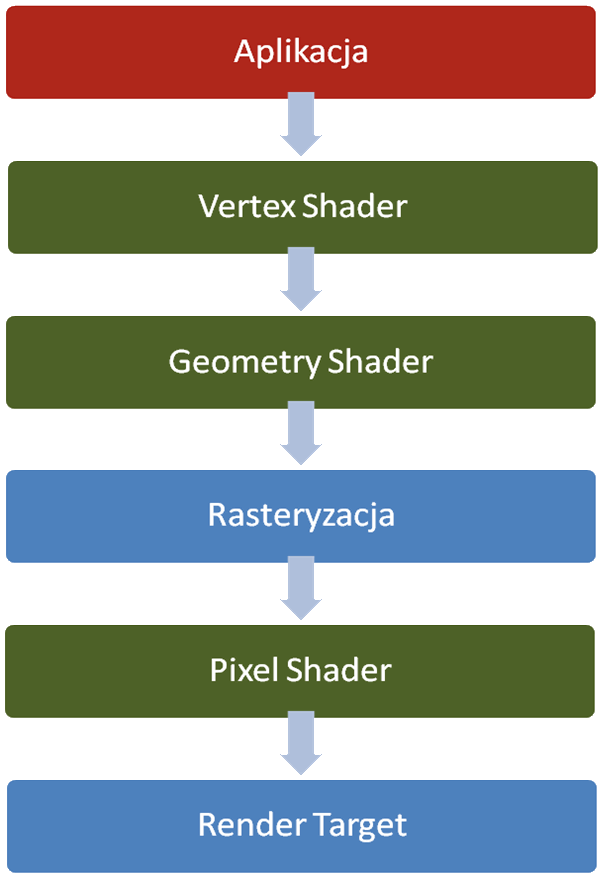
\includegraphics[height=7cm]{img/potok.png}
	\label{fig:potok}
	\end{figure}

}

\subsection{Organizacja pamięci}\label{sub:organizacja pamięci}
\frame{ \frametitle{Organizacja pamięci} \tableofcontents[currentsubsection] }

\frame
{
	\frametitle{Rodzaje pamięci na GPU}

	\begin{itemize}
	\item lokalna
	\item globalna
	\item tekstury
	\end{itemize}
}

\frame
{
	\frametitle{Organizacja pamięci}

	Część wspólna:
	\begin{itemize}
	\item pozycja
	\item promień
	\end{itemize}

	\pause
	Rodzaje buforów:

	\begin{itemize}
	\item bufory OpenGL
	\item bufory CUDA
	\end{itemize}

}

\begin{frame}[fragile]
	\frametitle{Implementacja buforów}
	\begin{verbatim}
//   * GFX
GBUF<int>    model;
GBUF<float>  emissive;

//   * COMMON
GBUF<float3>   pos;
GBUF<float>    radius;
GBUF<uint32_t> count;

//   * PHX
CBUF<float>    mass;
CBUF<float3>   velocity;
	\end{verbatim}
\end{frame}

\frame
{
	\frametitle{Dane graficzne}

	Dane dla silnika graficznego trzymane w pamięci tekstury.
	\begin{itemize}
	\item tekstura modeli
	\item tekstura tekstur
	\item tekstura normalnych
	\end{itemize}
}

\subsection{Deffered rendering}\label{sub:deffered rendering}
\frame{ \frametitle{Deffered rendering} \tableofcontents[currentsubsection] }

\frame
{
	\frametitle{Deffered rendering}

	\begin{itemize}
	\item generowanie bufora geometrii
	\item bufor jest proporcjonalny do wielkości ekranu
	\item finalny obrazek jest efektem postprocesingu g-bufora
	\item efekty graficzne (np. oświetlenie) są proporcjonalne obliczeniowo do wielkości bufora
	\end{itemize}
}

\frame
{
	\frametitle{g-bufor}

	\begin{figure}
	\centering
	\subfloat[color]{\label{fig:gcol}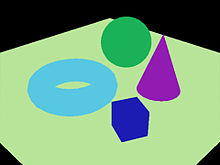
\includegraphics[width=0.3\textwidth]{img/gbuff_col.jpg}} \hspace{.0\textwidth}
	\subfloat[głębia]{\label{fig:gdepth}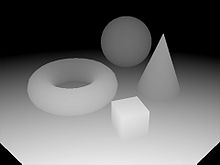
\includegraphics[width=0.3\textwidth]{img/gbuff_z.jpg}} \hspace{.0\textwidth} 
	\subfloat[normalne]{\label{fig:norm}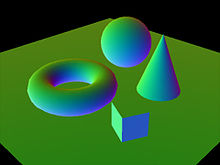
\includegraphics[width=0.3\textwidth]{img/gbuff_norm.jpg}} \hspace{.0\textwidth} \\
	\pause
	\subfloat[efekt]{\label{fig:gend}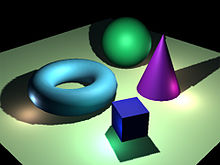
\includegraphics[width=0.3\textwidth]{img/gbuff_fin.jpg}}
	\label{fig:deffered_rednering}
	\end{figure}
	\setcounter{subfigure}{0}
}

\frame
{
	\frametitle{Wady i zalety}

	\begin{block}{Zalety}
	\begin{itemize}
		\item dobrze skalowalny ze względu na ilość dynamicznych świateł
		\item zmniejsza ilość obliczeń przy dużej ilości geometrii
		\item wydajny przy dużych otwartych przestrzeniach
	\end{itemize}
	\end{block}
	\begin{block}{Wady}
	\begin{itemize}
		\item duże bufory
		\item wymagane jest cieniowanie per piksel
		\item na starych komputerach potrzebne jest wiele przejść do wygenerowania g-bufora
	\end{itemize}
	\end{block}
}

\frame
{
	\frametitle{Przykłady użycia}

	Używany w wielu nowych grach:

	\begin{itemize}
	\item Stalker: Shadow of Chernobyl
	\item Grand Theft Auto IV
	\item StarCraft II
	\item CryEngine 3
	\end{itemize}
}

\section{Silnik graficzny}\label{sec:silnik graficzny}
\frame{ \frametitle{Silnik graficzny} \tableofcontents[currentsection] }

\subsection{Wymagania}\label{sub:wymagania}
\frame{ \frametitle{Wymagania} \tableofcontents[currentsubsection] }

\frame
{
	\frametitle{Wymagania}

	Wymagania funkcjonalne:
	\begin{description}
	\item[duże układy] - over 9000 planet
	\item[gwiazdy] - świecenie, rozmycie
	\item[komety] - warkocz pyłu
	\item[atmosfery] - półprzezroczyste powłoki wokół planet
	\end{description}
}

\frame
{
	\frametitle{Wejście}
	\begin{figure}
	\centering
	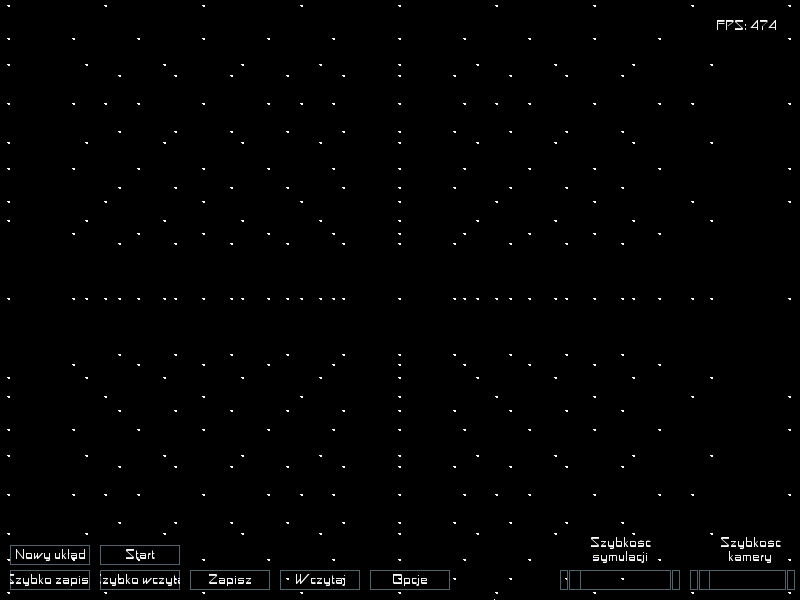
\includegraphics[height=7cm]{img/r_points.png}
	\label{fig:deffered_rednering}
	\end{figure}
}

\frame
{
	\frametitle{Wyjście}
	\begin{figure}
	\centering
	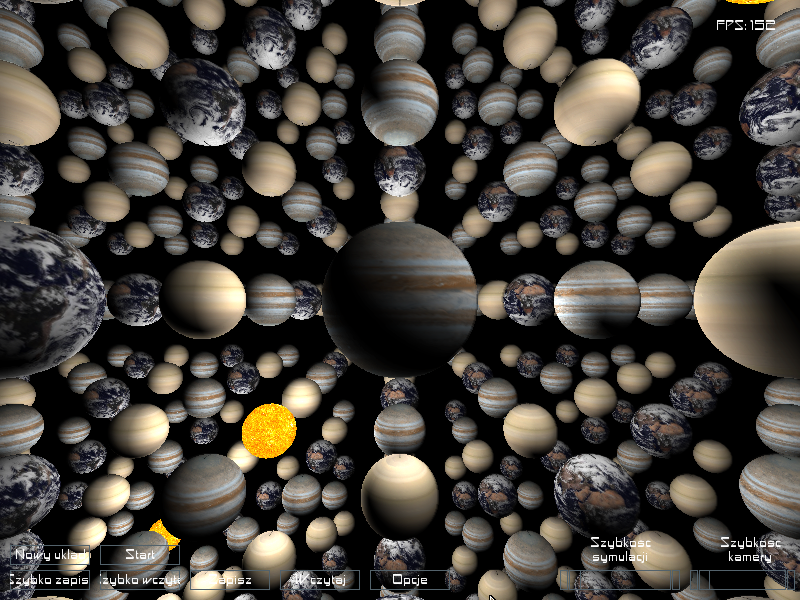
\includegraphics[height=7cm]{img/r_curr.png}
	\label{fig:deffered_rednering}
	\end{figure}

}

\subsection{Generowanie geometrii}\label{sub:generowanie geometrii}
\frame{ \frametitle{Generowanie geometrii} \tableofcontents[currentsubsection] }

\frame
{
	\frametitle{Geometria}

	\begin{figure}
	\centering
	\subfloat[60]   {\label{fig:sph0}
\includegraphics[width=0.25\textwidth]{img/sph_0.png}} \hspace{.0\textwidth}
	\subfloat[960]  {\label{fig:sph2}
\includegraphics[width=0.25\textwidth]{img/sph_2.png}} \hspace{.0\textwidth}
	\subfloat[61440]{\label{fig:sph5}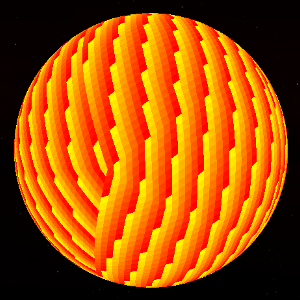
\includegraphics[width=0.25\textwidth]{img/sph_5.png}} \hspace{.0\textwidth} \\
	\pause
	\subfloat[4]    {\label{fig:sph_def}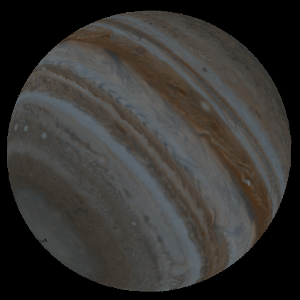
\includegraphics[width=0.25\textwidth]{img/sph_def.png}} \hspace{.0\textwidth} 
	\label{fig:deffered_rednering}
	\end{figure}
	\setcounter{subfigure}{0}
}

\subsection{Konstrukcja silnika}\label{sub:konstrukcja silnika}
\frame{ \frametitle{Konstrukcja silnika} \tableofcontents[currentsubsection] }

\frame
{
	\frametitle{Przejścia}

	Kolejne etapy wykonywane przez silnik graficzny:

	\begin{enumerate}
	\item generowanie g-bufora
	\item światła ambient i emissive
	\item światła dynamiczne
	\item rozmycie 
	\item efekt atmosfery
	\item efekt komet
	\end{enumerate}
}

\section{Silnik fizyczny}\label{sec:silnik fizyczny}
\frame{ \frametitle{Silnik fizyczny} \tableofcontents[currentsection] }

\frame
{
	\frametitle{Kiedyś-będzie-zrobiony silnik}
}

%\setbeamercolor{normal text}{bg=black}

%\setbeamertemplate{background}{\includegraphics[width=\paperwidth]{img/mirabella.jpg}}
%\frame { }

%\setbeamertemplate{background}{\includegraphics[width=\paperwidth]{img/sokol_maltanski.jpg}}
%\frame { }

\end{document}

